\documentclass[]{article}\usepackage[]{graphicx}\usepackage[]{color}
%% maxwidth is the original width if it is less than linewidth
%% otherwise use linewidth (to make sure the graphics do not exceed the margin)
\makeatletter
\def\maxwidth{ %
  \ifdim\Gin@nat@width>\linewidth
    \linewidth
  \else
    \Gin@nat@width
  \fi
}
\makeatother

\definecolor{fgcolor}{rgb}{0.345, 0.345, 0.345}
\newcommand{\hlnum}[1]{\textcolor[rgb]{0.686,0.059,0.569}{#1}}%
\newcommand{\hlstr}[1]{\textcolor[rgb]{0.192,0.494,0.8}{#1}}%
\newcommand{\hlcom}[1]{\textcolor[rgb]{0.678,0.584,0.686}{\textit{#1}}}%
\newcommand{\hlopt}[1]{\textcolor[rgb]{0,0,0}{#1}}%
\newcommand{\hlstd}[1]{\textcolor[rgb]{0.345,0.345,0.345}{#1}}%
\newcommand{\hlkwa}[1]{\textcolor[rgb]{0.161,0.373,0.58}{\textbf{#1}}}%
\newcommand{\hlkwb}[1]{\textcolor[rgb]{0.69,0.353,0.396}{#1}}%
\newcommand{\hlkwc}[1]{\textcolor[rgb]{0.333,0.667,0.333}{#1}}%
\newcommand{\hlkwd}[1]{\textcolor[rgb]{0.737,0.353,0.396}{\textbf{#1}}}%
\let\hlipl\hlkwb

\usepackage{framed}
\makeatletter
\newenvironment{kframe}{%
 \def\at@end@of@kframe{}%
 \ifinner\ifhmode%
  \def\at@end@of@kframe{\end{minipage}}%
  \begin{minipage}{\columnwidth}%
 \fi\fi%
 \def\FrameCommand##1{\hskip\@totalleftmargin \hskip-\fboxsep
 \colorbox{shadecolor}{##1}\hskip-\fboxsep
     % There is no \\@totalrightmargin, so:
     \hskip-\linewidth \hskip-\@totalleftmargin \hskip\columnwidth}%
 \MakeFramed {\advance\hsize-\width
   \@totalleftmargin\z@ \linewidth\hsize
   \@setminipage}}%
 {\par\unskip\endMakeFramed%
 \at@end@of@kframe}
\makeatother

\definecolor{shadecolor}{rgb}{.97, .97, .97}
\definecolor{messagecolor}{rgb}{0, 0, 0}
\definecolor{warningcolor}{rgb}{1, 0, 1}
\definecolor{errorcolor}{rgb}{1, 0, 0}
\newenvironment{knitrout}{}{} % an empty environment to be redefined in TeX

\usepackage{alltt}
\usepackage[landscape, margin=0.1in]{geometry}
%\usepackage[margin=0.1in]{geometry}
%\usepackage[left=0.1in, bottom=0.1in, top=0.1in, right=0.3in]{geometry}
\usepackage{grid-system}
\renewcommand{\familydefault}{\sfdefault}
\usepackage{setspace}			% \doublespacing
\usepackage{graphicx}
\usepackage{graphbox} 		% loads graphicx package			Not sure if I'm using this
\usepackage{xcolor}				% textbox colors (I think being used by \fcolorbox)
\usepackage{hyperref}
\hypersetup{
	colorlinks=true,
	linkcolor=blue,
	filecolor=magenta, 
	urlcolor=blue,
  linkbordercolor=cyan, %hyperlink border
  pdfborderstyle={/S/U/W 1} % border style will be underline of width 1 pt
}

\usepackage{fancyhdr}
\usepackage{lastpage}		% For \pageref{LastPage}
\pagestyle{fancy}
\fancyhf{}
% Manually adjust the vertical space in the header and footer to account for narrow 
%   margins. This is kludgy.
%\rhead{\vspace{1.2cm} {\footnotesize \emph{Report Version 1.1, Updated 2019-02-15}}}
\rfoot{\vspace{-1.5cm} Page \thepage \hspace{1pt} of \pageref*{LastPage}}
\renewcommand{\headrulewidth}{0pt}		% Get rid of fancyhdr's vertical lines
\renewcommand{\footrulewidth}{0pt}		% Get rid of fancyhdr's vertical lines

\usepackage{parskip}		% Bullets close together

%\usepackage{lmodern}		% for custom font size

% Using this instead of base itemize because it allows for easier customization of 
%   margins:
\usepackage{enumitem}			% [leftmargin=*]
%\renewcommand\labelitemi{\tiny$\bullet$}		% smaller itemize bullets

\setlength{\fboxsep}{5pt}		% fcolorbox margins
%%%%%%%%%%%%%%%%%%%%%%%%%%%%%%%%%%%%%%%%%%%%%%%%%%%%%%%%%%%%%%
\IfFileExists{upquote.sty}{\usepackage{upquote}}{}
\begin{document}




%%%% Cover page:
\begin{Row}
  \begin{Cell}{3}
    \begin{center}
      \vspace{15pt}
      
\includegraphics[width=3cm,trim=0 0 0 0,clip,align=m]{figures/IEP_logo.PNG}
    \end{center}
  \end{Cell}
  \begin{Cell}{10}
    \begin{center}
      {\fontsize{5cm}{5.5cm}\selectfont Winter 2017-2018} \\
      \vspace{15pt}
      {\Huge IEP Status and Trends Report} \\
      \vspace{15pt}
      {\large 
        Interagency Ecological Program for the San Francisco Estuary

        This report shows trends in water quality, plankton, and fish across multiple IEP surveys for December of 2017, January and February of 2018.
      }
    \end{center}
  \end{Cell}
  \begin{Cell}{3}
    \begin{center}
    \end{center}
  \end{Cell}  
\end{Row}

\vspace{30pt}

\begin{Row}
  \begin{Cell}{2}
    \begin{center}
    \end{center}
  \end{Cell}
  \begin{Cell}{5}
    \begin{center}
      {\Huge Regions of the Estuary}
    \end{center}
  \end{Cell}
  \begin{Cell}{5}
    \begin{center}
      {\Huge Delta Outflow}
    \end{center}
  \end{Cell}
\end{Row}

\begin{Row}
  \begin{Cell}{2}
    \begin{center}
      {\bf {\Large Contents}} \\ \vspace{7pt}
      \hyperlink{page:secchi}{{\Large Secchi Depth}} \\ \vspace{7pt}
      \hyperlink{page:temperature}{{\Large Temperature}} \\ \vspace{7pt}
      \hyperlink{page:chlorophyll}{{\Large Chlorophyll}} \\ \vspace{7pt}
      \hyperlink{page:zooplankton}{{\Large Zooplankton}} \\ \vspace{7pt}
      \hyperlink{page:fish}{{\Large Fish}} \\ \vspace{7pt}
      \hyperlink{page:recenttrends}{{\Large Recent Trends}} \\ \vspace{7pt}
    \end{center}
  \end{Cell}
  \begin{Cell}{5}
    \begin{center}
      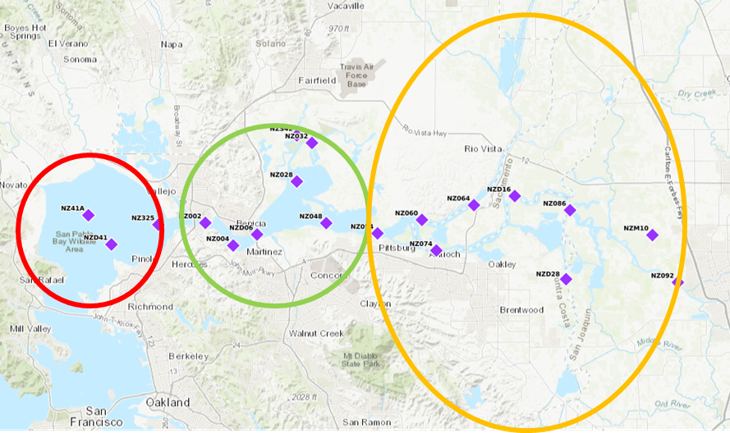
\includegraphics[width=10cm,trim=0 0 0 0,clip,align=m]{figures/region_map_2.png}
      \vspace{10pt}
      {\large 
        \begin{itemize}[leftmargin=1cm,rightmargin=1cm]
          \item San Pablo Bay is salty, similar to San Francisco Bay, with influence from 
          the Pacific Ocean.
          \item Suisun is brackish in the summer, fresher in the winter/spring, and 
          contains a lot of wetlands.
          \item The Delta is fresh, with many distributary channels.
        \end{itemize}
      }
    \end{center}
  \end{Cell}  
  \begin{Cell}{5}
    \begin{center}
      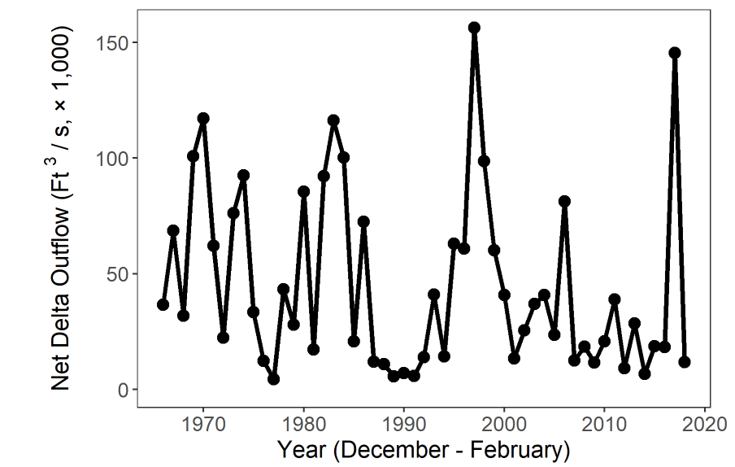
\includegraphics[width=10cm,trim=0 0 0 0,clip,align=m]{figures/outflow_tmp.png}
      \vspace{10pt}
      {\large 
        \begin{itemize}[leftmargin=1cm,rightmargin=1cm]
          \item Freshwater flow is one of the controlling factors in the estuary.
          \item Winter flow is driven primarily by rainfall and upstream dam releases.
        \end{itemize}
      }
    \end{center}
  \end{Cell}
\end{Row}

\vspace{30pt}

\begin{Row}
  \begin{Cell}{1}
    \begin{center}
      {\large DISCLAIMER: Use this data at your own risk}
    \end{center}
  \end{Cell}
\end{Row}


\newpage


%%%% Secchi Depth:
\hypertarget{page:secchi}{}
\begin{Row}
  \begin{Cell}{1}
    \begin{center}
      {\Large Interagency Ecological Program Status \& Trends 2017-2018 Winter Season Report}
    \end{center}
  \end{Cell}
\end{Row}

\begin{Row}
  \begin{Cell}{1}
    \begin{center}
      {\Huge Secchi Depth}
    \end{center}
  \end{Cell}
\end{Row}

\begin{Row}
  \begin{Cell}{8}
    \begin{center}
      {\large 
        \begin{itemize}[leftmargin=2cm,rightmargin=2cm]
          \item Organisms in this ecosystem are adapted to high turbidity conditions, 
          and reductions in turbidity can have many negative ecological effects. Higher 
          values for Secchi depth indicate lower turbidity.
          \item Secchi depth is measured monthly by DWR’s Environmental monitoring 
          program by dropping a black-and-white disk in the water until it disappears.
        \end{itemize}
      }
    \end{center}
  \end{Cell}

  \begin{Cell}{2}
    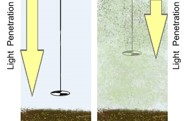
\includegraphics[width=6cm,align=m]{figures/secchi/secchi_diagram.jpg}
  \end{Cell}
\end{Row}

\vspace{30pt}

\begin{Row}
  \begin{Cell}{4}
    \begin{center}
      {\Large {\bf San Pablo Bay}}
    \end{center}
  \end{Cell}
  \begin{Cell}{4}
    \begin{center}
      {\Large {\bf Suisun Bay}}
    \end{center}
  \end{Cell}
  \begin{Cell}{4}
    \begin{center}
      {\Large {\bf The Delta}}
    \end{center}
  \end{Cell}
\end{Row}

\begin{Row}
  \begin{Cell}{4}
    \begin{center}
      \includegraphics[width=8cm,align=m]{figures/secchi/placeholder_fig.png}
      \vspace{0.5cm}
      \begin{itemize}[leftmargin=1.5cm,rightmargin=1cm]
        \item San Pablo bay is pretty clear.
      \end{itemize}
    \end{center}
  \end{Cell}

  \begin{Cell}{4}
    \begin{center}
      \includegraphics[width=8cm,align=m]{figures/secchi/placeholder_fig.png}
      \vspace{0.5cm}
      \begin{itemize}[leftmargin=1.5cm,rightmargin=1cm]
        \item Suisun Bay is pretty murky (low Secchi depth).
      \end{itemize}
    \end{center}
  \end{Cell}

  \begin{Cell}{4}
    \begin{center}
      \includegraphics[width=8cm,align=m]{figures/secchi/placeholder_fig.png}
      \vspace{0.5cm}
      \begin{itemize}[leftmargin=1.5cm,rightmargin=1cm]
        \item The Delta has been getting clearer over time.
      \end{itemize}
    \end{center}
  \end{Cell}
\end{Row}


\newpage


%%%% Temperature:
\hypertarget{page:temperature}{}
\begin{Row}
  \begin{Cell}{1}
    \begin{center}
      {\Large Interagency Ecological Program Status \& Trends 2017-2018 Winter Season Report}
    \end{center}
  \end{Cell}
\end{Row}

\begin{Row}
  \begin{Cell}{1}
    \begin{center}
      {\Huge Temperature}
    \end{center}
  \end{Cell}
\end{Row}

\begin{Row}
  \begin{Cell}{8}
    \begin{center}
      {\large 
        \begin{itemize}[leftmargin=2cm,rightmargin=2cm]
          \item Temperature is monitored monthly by DWR's Environmental Monitoring 
          Program.
          \item Most fish have temperature tolerances necessary for growth and 
          reproduction.
          \item Increasing winter temperatures may lower Delta Smelt fecundity.
        \end{itemize}
      }
    \end{center}
  \end{Cell}

  \begin{Cell}{2}
    
\includegraphics[width=6cm,align=m]{figures/temperature/temperature_graphic.png}
  \end{Cell}
\end{Row}

\vspace{30pt}

\begin{Row}
  \begin{Cell}{4}
    \begin{center}
      {\Large {\bf San Pablo Bay}}
    \end{center}
  \end{Cell}
  \begin{Cell}{4}
    \begin{center}
      {\Large {\bf Suisun Bay}}
    \end{center}
  \end{Cell}
  \begin{Cell}{4}
    \begin{center}
      {\Large {\bf The Delta}}
    \end{center}
  \end{Cell}
\end{Row}

\begin{Row}
  \begin{Cell}{4}
    \begin{center}
      \includegraphics[width=8cm,align=m]{figures/temperature/placeholder_fig.png}
      \vspace{0.5cm}
      \begin{itemize}[leftmargin=1.5cm,rightmargin=1cm]
        \item San Pablo Bay is slightly warmer than the Delta in the winter.
      \end{itemize}
    \end{center}
  \end{Cell}

  \begin{Cell}{4}
    \begin{center}
      \includegraphics[width=8cm,align=m]{figures/temperature/placeholder_fig.png}
      \vspace{0.5cm}
      \begin{itemize}[leftmargin=1.5cm,rightmargin=1cm]
        \item Suisun Bay is usually similar to the Delta.
      \end{itemize}
    \end{center}
  \end{Cell}

  \begin{Cell}{4}
    \begin{center}
      \includegraphics[width=8cm,align=m]{figures/temperature/placeholder_fig.png}
      \vspace{0.5cm}
      \begin{itemize}[leftmargin=1.5cm,rightmargin=1cm]
        \item Delta temperatures are closely linked to air temperature.
      \end{itemize}
    \end{center}
  \end{Cell}
\end{Row}


\newpage


%%%% Chlorophyll:
\hypertarget{page:chlorophyll}{}
\begin{Row}
  \begin{Cell}{1}
    \begin{center}
      {\Large Interagency Ecological Program Status \& Trends 2017-2018 Winter Season Report}
    \end{center}
  \end{Cell}
\end{Row}

\begin{Row}
  \begin{Cell}{1}
    \begin{center}
      {\Huge Chlorophyll}
    \end{center}
  \end{Cell}
\end{Row}

\begin{Row}
  \begin{Cell}{8}
    \begin{center}
      {\large 
        \begin{itemize}[leftmargin=2cm,rightmargin=2cm]
          \item Chlorophyll is an indicator of phytoplankton production, which tends 
          to be low during the winter.
          \item Phytoplankton are the base of the pelagic food web. It is sampled 
          monthly by DWR's Environmental Monitoring Program.
          \item The invasive clam {\em Potamocorbula amurensis} caused a decline in 
          phytoplankton and zooplankton -- especially in Suisun Bay.
        \end{itemize}
      }
    \end{center}
  \end{Cell}

  \begin{Cell}{2}
    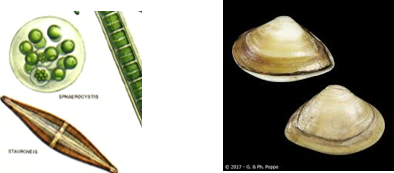
\includegraphics[width=6cm,align=m]{figures/chlorophyll/chlorophyll_pics.png}
  \end{Cell}
\end{Row}

\vspace{30pt}

\begin{Row}
  \begin{Cell}{4}
    \begin{center}
      {\Large {\bf San Pablo Bay}}
    \end{center}
  \end{Cell}
  \begin{Cell}{4}
    \begin{center}
      {\Large {\bf Suisun Bay}}
    \end{center}
  \end{Cell}
  \begin{Cell}{4}
    \begin{center}
      {\Large {\bf The Delta}}
    \end{center}
  \end{Cell}
\end{Row}

\begin{Row}
  \begin{Cell}{4}
    \begin{center}
      \includegraphics[width=8cm,align=m]{figures/chlorophyll/placeholder_fig.png}
      \vspace{0.5cm}
      \begin{itemize}[leftmargin=1.5cm,rightmargin=1cm]
        \item Winter chlorophyll has been consistently low in San Pablo Bay.
      \end{itemize}
    \end{center}
  \end{Cell}

  \begin{Cell}{4}
    \begin{center}
      \includegraphics[width=8cm,align=m]{figures/chlorophyll/placeholder_fig.png}
      \vspace{0.5cm}
      \begin{itemize}[leftmargin=1.5cm,rightmargin=1cm]
        \item The clam invasion lowered chlorophyll in Suisun more than other regions.
      \end{itemize}
    \end{center}
  \end{Cell}

  \begin{Cell}{4}
    \begin{center}
      \includegraphics[width=8cm,align=m]{figures/chlorophyll/placeholder_fig.png}
      \vspace{0.5cm}
      \begin{itemize}[leftmargin=1.5cm,rightmargin=1cm]
        \item Winter chlorophyll levels have been consistently low in the Delta.
      \end{itemize}
    \end{center}
  \end{Cell}
\end{Row}


\newpage


%%%% Zooplankton:
\hypertarget{page:zooplankton}{}
\begin{Row}
  \begin{Cell}{1}
    \begin{center}
      {\Large Interagency Ecological Program Status \& Trends 2017-2018 Winter Season Report}
    \end{center}
  \end{Cell}
\end{Row}

\begin{Row}
  \begin{Cell}{1}
    \begin{center}
      {\Huge Zooplankton}
    \end{center}
  \end{Cell}
\end{Row}

\begin{Row}
  \begin{Cell}{8}
    \begin{center}
      {\large 
        \begin{itemize}[leftmargin=2cm,rightmargin=2cm]
          \item Zooplankton is sampled monthly by the CDFW/DWR Environmental Monitoring 
          Program, but sampling in winter did not begin until 1995. 
          \item Zooplankton are an important food source for pelagic fish. Calanoid 
          copepods and mysids are good fish food. Cyclopoid copepods are not as good 
          for fish food.
          \item Biomass tends to be low in the winter.
        \end{itemize}
      }
    \end{center}
  \end{Cell}

  \begin{Cell}{2}
    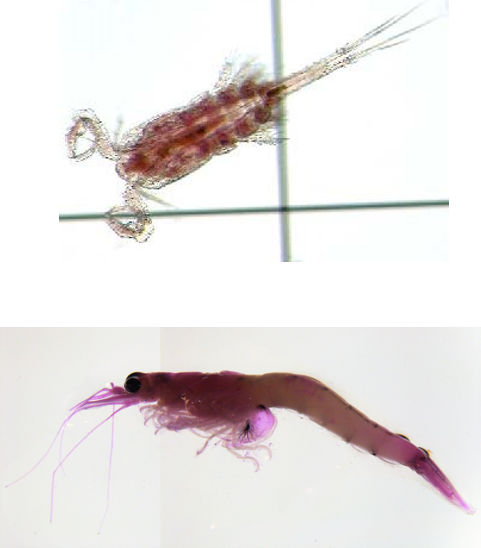
\includegraphics[width=5cm,align=m]{figures/zoop/bug0.png}
  \end{Cell}
\end{Row}

\vspace{30pt}

\begin{Row}
  \begin{Cell}{4}
    \begin{center}
      {\Large {\bf San Pablo Bay}}
    \end{center}
  \end{Cell}
  \begin{Cell}{4}
    \begin{center}
      {\Large {\bf Suisun Bay}}
    \end{center}
  \end{Cell}
  \begin{Cell}{4}
    \begin{center}
      {\Large {\bf The Delta}}
    \end{center}
  \end{Cell}
  \begin{Cell}{3}
    \begin{center}
    \end{center}
  \end{Cell}  
\end{Row}

%\vspace{-100pt}

\begin{Row}
  \begin{Cell}{4}
    \begin{center}
      \includegraphics[width=7cm,align=m]{figures/zoop/placeholder_fig.png}
      \begin{itemize}[leftmargin=1.5cm,rightmargin=1cm,topsep=10pt]
        \item San Pablo Bay is dominated by calanoid copepods.
      \end{itemize}
    \end{center}
  \end{Cell}

  \begin{Cell}{4}
    \begin{center}
      \includegraphics[width=7cm,align=m]{figures/zoop/placeholder_fig.png}
      \begin{itemize}[leftmargin=1.5cm,rightmargin=1cm,topsep=10pt]
        \item Suisun has a lot of cyclopoid copepods.
      \end{itemize}
    \end{center}
  \end{Cell}

  \begin{Cell}{4}
    \begin{center}
      \includegraphics[width=7cm,align=m]{figures/zoop/placeholder_fig.png}
      \begin{itemize}[leftmargin=1.5cm,rightmargin=1cm,topsep=10pt]
        \item The Delta has low zooplankton abundance during the winter.
      \end{itemize}
    \end{center}
  \end{Cell}
  
  \begin{Cell}{3}
    \begin{center}
      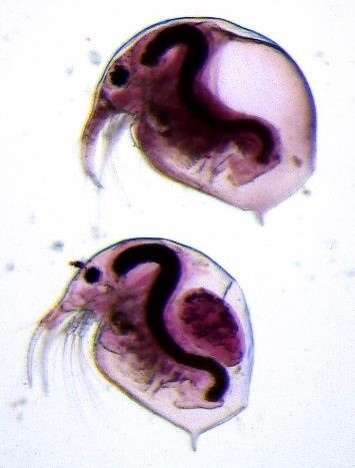
\includegraphics[width=4cm,trim=0 0 0 0,clip,align=m]{figures/zoop/bug3.jpg}
    \end{center}
  \end{Cell}  
\end{Row}


\newpage


%%%% Fish:
\hypertarget{page:fish}{}
\begin{Row}
  \begin{Cell}{1}
    \begin{center}
      {\Large Interagency Ecological Program Status \& Trends 2017-2018 Winter Season Report}
    \end{center}
  \end{Cell}
\end{Row}

\begin{Row}
  \begin{Cell}{1}
    \begin{center}
      {\Huge Fish}
    \end{center}
  \end{Cell}
\end{Row}

\begin{Row}
  \begin{Cell}{1}
    \begin{center}
      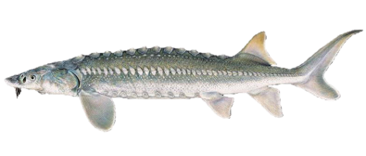
\includegraphics[width=7cm,align=m]{figures/otherfish/white_sturgeon_fig.png}
    \end{center}
  \end{Cell}
  \begin{Cell}{1}
    \begin{center}
      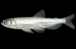
\includegraphics[align=m]{figures/smelt/photo_longfin_smelt.png}
    \end{center}
  \end{Cell}
\end{Row}

\begin{Row}
  \begin{Cell}{1}
    \begin{center}
      {\bf {\large White Sturgeon – Bay Study}}
    \end{center}
  \end{Cell}
  \begin{Cell}{1}
    \begin{center}
      {\bf {\large Longfin Smelt – Bay Study}}
    \end{center}
  \end{Cell}
\end{Row}

\begin{Row}
  \begin{Cell}{1}
    {\large 
      \begin{center}
        \includegraphics[width=10cm,align=m]{figures/otherfish/placeholder_fig.png}
        \begin{itemize}[leftmargin=1.5cm,rightmargin=1cm,topsep=10pt]
          \item White sturgeon support a recreational fishery.
          \item Juvenile sturgeon are caught in CDFW's San Francisco Bay Study's otter trawl.
        \end{itemize}
      \end{center}
    }
  \end{Cell}
  \begin{Cell}{1}
    {\large 
      \begin{center}
        \includegraphics[width=10cm,align=m]{figures/otherfish/placeholder_fig.png}
        \begin{itemize}[leftmargin=1.5cm,rightmargin=1cm,topsep=10pt]
          \item Longfin Smelt are listed as Threatened under CESA and have been in decline 
          since the early 2000s. 
          \item Longfin Smelt are sampled by CDFW’s San Francisco Bay Study's midwater trawl.
        \end{itemize}
      \end{center}
    }
  \end{Cell}
\end{Row}


\newpage


%%%% Recent Trends:
\hypertarget{page:recenttrends}{}
\begin{Row}
  \begin{Cell}{1}
    \begin{center}
      {\Large Interagency Ecological Program Status \& Trends 2017-2018 Winter Season Report}
    \end{center}
  \end{Cell}
\end{Row}

\begin{Row}
  \begin{Cell}{1}
    \begin{center}
      {\Huge Recent Trends}
    \end{center}
  \end{Cell}
\end{Row}

\begin{Row}
  \begin{Cell}{1}
    \begin{center}
      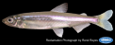
\includegraphics[width=3cm,align=m]{figures/smelt/photo_delta_smelt.png}
    \end{center}
  \end{Cell}
  \begin{Cell}{1}
    \begin{center}
    \end{center}
  \end{Cell}  
  \begin{Cell}{1}
    \begin{center}
      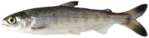
\includegraphics[align=m]{figures/salmon/photo_salmon.png}
    \end{center}
  \end{Cell}
\end{Row}

\begin{Row}
  \begin{Cell}{1}
    \begin{center}
      {\bf {\large Delta Smelt – SKT}}
    \end{center}
  \end{Cell}
  \begin{Cell}{1}
    \begin{center}
      {\bf {\large Winter Run Chinook – RBDD}}
    \end{center}
  \end{Cell}  
  \begin{Cell}{1}
    \begin{center}
      {\bf {\large Juvenile Chinook – DJFMP}}
    \end{center}
  \end{Cell}
\end{Row}

\begin{Row}
  \begin{Cell}{1}
    {\large 
      \begin{center}
        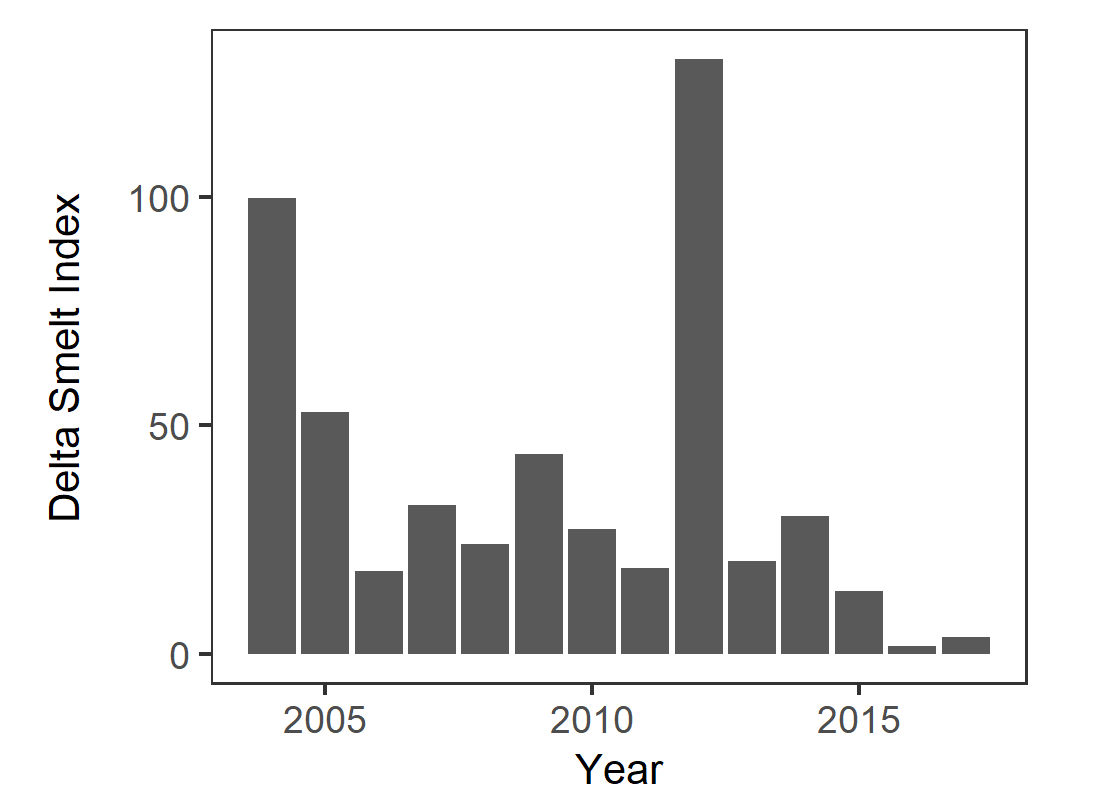
\includegraphics[width=9cm,align=m]{figures/smelt/skt_dsm_fig.png}
        \begin{itemize}[leftmargin=1.5cm,rightmargin=1cm,topsep=10pt]
          \item Delta Smelt are ESA listed as Threatened, CESA listed as Endangered and 
          have been in decline since the early 2000s
          \item CDFW's Spring Kodiak Trawl is designed to monitor adult Delta Smelt 
          from January-March.
        \end{itemize}
      \end{center}
    }
  \end{Cell}
  \begin{Cell}{1}
    {\large 
      \begin{center}
        % Replace this figure .................
        \includegraphics[width=9cm,align=m]{figures/smelt/placeholder_fig.png}
        \begin{itemize}[leftmargin=1.5cm,rightmargin=1cm,topsep=10pt]
          \item Juvenile Chinook pass Red Bluff Diversion Dam as they migrate from 
          spawning grounds to the ocean.
          \item Sampling at the dam provides an estimate of production in the upper 
          watershed.
        \end{itemize}
      \end{center}
    }
  \end{Cell}
  \begin{Cell}{1}
    {\large 
      \begin{center}
        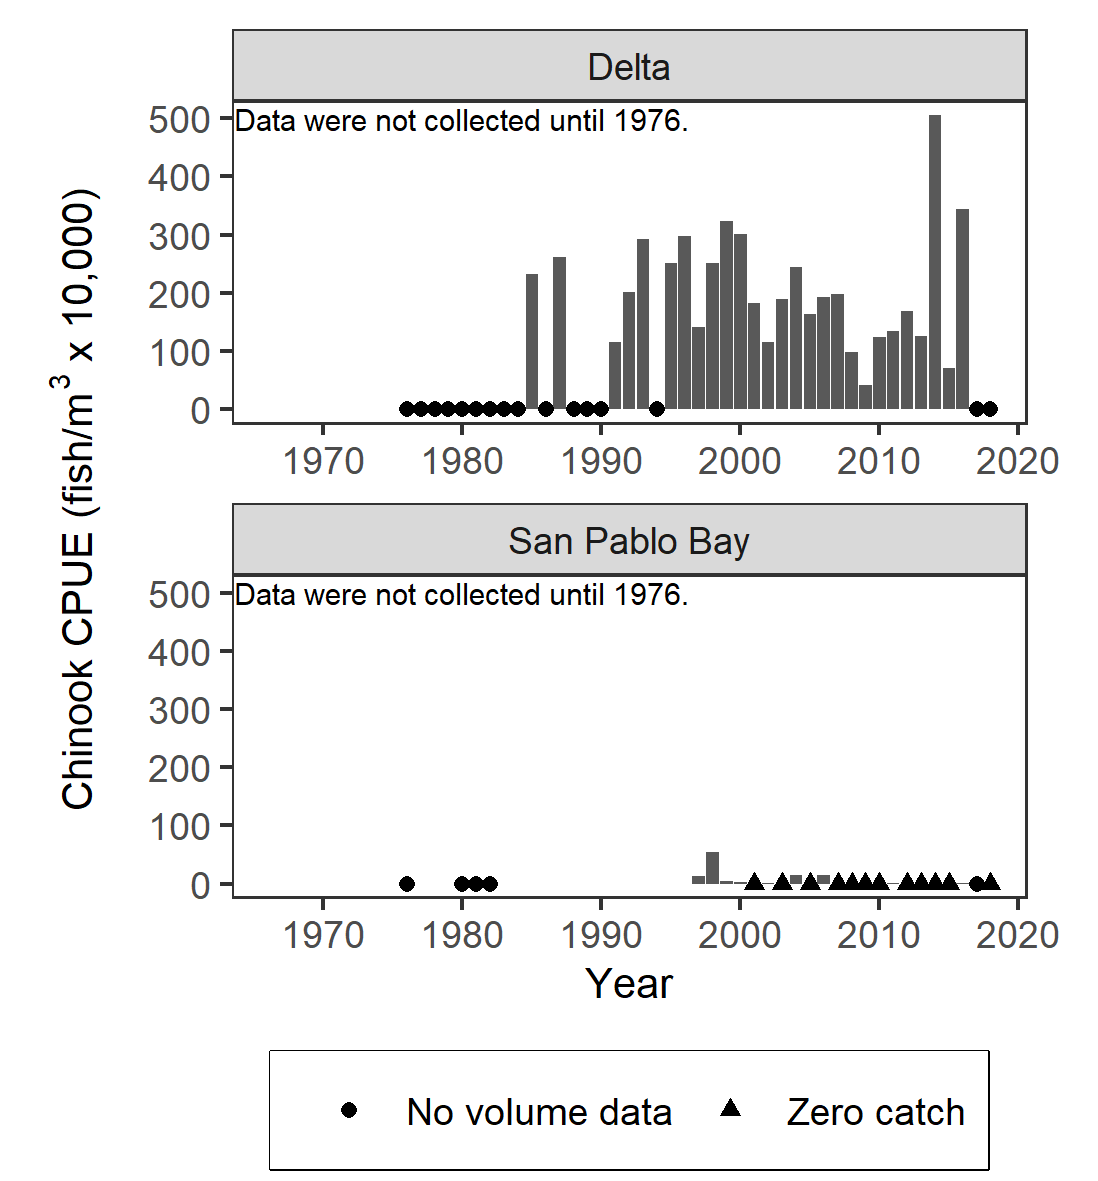
\includegraphics[width=9cm,align=m]{figures/salmon/djfmp_chn_fig_1966.png}
        \begin{itemize}[leftmargin=1.5cm,rightmargin=1cm,topsep=10pt]
          \item USFWS's Delta Juvenile Fish Monitoring Program runs beach seines to 
          show landscape patterns of juvenile Chinook Salmon.
          \item Researchers use these patterns to determine differences in salmon 
          life-history.
        \end{itemize}
      \end{center}
    }
  \end{Cell}
  
\end{Row}


\end{document}
